\documentclass[english]{article}

\usepackage[latin9]{inputenc}
\usepackage[letterpaper]{geometry}
\geometry{verbose,tmargin=1in,bmargin=1in,lmargin=1in,rmargin=1in}
\usepackage{amsmath}
\usepackage{amssymb}
\usepackage{graphicx}

\title{CIS 520, Machine Learning, Fall 2015: Assignment 4 \\
Due: Thursday, October 15th, 11:59pm, PDF to Canvas\\}
\date{}

\begin{document}
\maketitle

\section*{Boosting and MDL}
\label{sec:boosting}

\subsection*{1. Analyzing the training error of boosting}

Consider the AdaBoost algorithm you saw in class. In this question
we will try to analyze the training error of boosting.

\begin{enumerate}
\item Given a set of $m$ examples, $(x_i,y_i)$ ($y_i$ is
  the class label of $x_i$), $i=1,\ldots,m$, let $h_t(x)$ be the weak
  classifier obtained at step $t$, and let $\alpha_t$ be its
  weight. Recall that the final classifier is
  \[
  H(x) = \mbox{sign} (f(x)), \mbox{ where } f(x) = \sum_{t=1}^T
  \alpha_t h_t(x).
  \]
  Show that the training error of the final classifier can be bounded
  from above by an exponential loss function:
  \[
  \frac{1}{m} \sum_{i=1}^m I(H(x_i) \neq y_i) \leq \frac{1}{m}
  \sum_{i=1}^m \exp( -f(x_i) y_i),
  \]
  where $I(a=b)$ is the indicator function. It is equal to 1 if $a=b$,
  and 0 otherwise

  {\em Hint}: $e^{-x} \geq 1 \Leftrightarrow x \leq 0$. 


\item 
  Remember that
  \[D_{t+1}(i)=\frac{D_t(i)\exp(-\alpha_ty_ih_t(x_i))}{Z_t}\] Use this
  recursive definition to prove the following.
  \begin{equation}
    \label{boosting:upper bound} \frac{1}{m} \sum_{i=1}^m \exp( -f(x_i)
    y_i) = \prod_{t=1}^T Z_t,
  \end{equation}
  where $Z_t$ is the normalization factor for distribution $D_{t+1}$:
  \begin{equation}
    \label{boosting:normalization_expression} Z_t = \sum_{i=1}^m D_t(i)
    \exp(-\alpha_t y_i h_t(x_i)).
  \end{equation}

  {\em Hint}: Remember that $e^{\sum_i g_i}=\prod_i
  e^{g_i}$,$D_1(i)=\frac{1}{m}$, and that $\sum_i D_{t+1}(i) = 1$.


\item  \begin{equation} \frac{1}{m} \sum_{i=1}^m \exp( -f(x_i)
    y_i) = \prod_{t=1}^T Z_t,
  \end{equation}
 suggests that the
  training error can be reduced rapidly by greedily optimizing $Z_t$
  at each step.  You have shown that the error is bounded from above:
  \[
  \epsilon_{training} \leq \prod_{t=1}^T Z_t.
  \]
  Observe that $Z_1, \dots, Z_{t-1}$ are determined by the first
  $(t-1)$ rounds of boosting, and we cannot change them on round $t$.
  A greedy step we can take to minimize the training error bound on
  round $t$ is to minimize $Z_t$.

  In this question, you will prove that for binary weak classifiers,
  $Z_t$ from 
\begin{equation}
    \label{boosting:normalization_expression} Z_t = \sum_{i=1}^m D_t(i)
    \exp(-\alpha_t y_i h_t(x_i)).
  \end{equation}
 is minimized by picking $\alpha_t$ as:
  \begin{equation}\label{eq:alpha}
    \alpha_t^* = \frac{1}{2}\log\left( \frac{1 - \epsilon_t}{\epsilon_t}
    \right),
  \end{equation}
  where $\epsilon_t$ is the training error of weak classifier $h_t$
  for the weighted dataset:
  \[
  \epsilon_t = \sum_{i=1}^m D_{t}(i) I(h_t(x_i) \neq y_i).
  \]
  where $I$ is the indicator function. For this proof, only consider
  the simplest case of binary classifiers, i.e. the output of $h_t(x)$
  is binary, \{$-1,+1$\}.

  For this special class of classifiers, first show that the
  normalizer $Z_t$ can be written as:
  \[
  Z_t = (1-\epsilon_t)\exp(-\alpha_t) + \epsilon_t\exp(\alpha_t).
  \]

  {\em Hint}: Consider the sums over correctly and incorrectly
  classified examples separately.


\item  Now, prove that the value of $\alpha_t$ that
  minimizes this definition of $Z_t$ is given by Equation
 \begin{equation}
    \alpha_t^* = \frac{1}{2}\log\left( \frac{1 - \epsilon_t}{\epsilon_t}
    \right).
  \end{equation}


\item Prove that for the above value of $\alpha_t$ we
  have $Z_t = 2\sqrt{\epsilon_t(1-\epsilon_t)}$.


\item Furthermore, let $\epsilon_t=\frac{1}{2}-\gamma_t$
  and prove that $Z_t\leq \exp(-2\gamma_t^2)$.  Therefore, we will
  know
  \begin{equation*}
    \epsilon_{training} \le \prod_tZ_t \le
    \exp(-2\sum_t\gamma_t^2).
  \end{equation*}

  {\em Hint}: $\log(1-x)\leq -x$ for $0<x\leq 1$.

\item If each weak classifier is slightly better than
  random, so that $\gamma_t \ge \gamma$, for some $\gamma > 0$, then
  the training error drops exponentially fast in $T$, i.e.
  \[\epsilon_{training}\leq \exp(-2T\gamma^2).\]

  Argue that in each round of boosting, there always exists a weak
  classifier $h_t$ such that its training error on the weighted
  dataset $\epsilon_t \le 0.5$.


\item Show that for $\epsilon_t = 0.5$ the training error
  can get ``stuck'' above zero.  {\em Hint}: $D_t(i)$s may get stuck.
\end{enumerate}

\subsection*{2. Adaboost on a toy dataset}

\begin{figure}[t]
  \begin{center}
    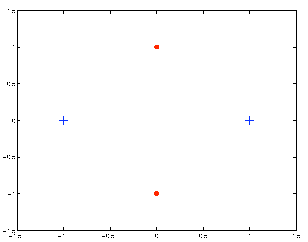
\includegraphics[width=2in]{images/toydata}
    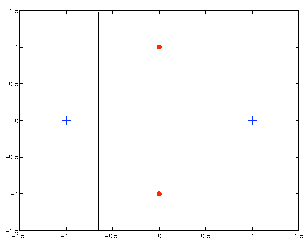
\includegraphics[width=2in]{images/toydata_with_h1}
  \end{center}
  \caption{a) Toy data in Question~\ref{sec:boosting}. b) $h_1$ in Question~\ref{sec:boosting}}
  \label{fig:toydata}
\end{figure}

Now we will apply Adaboost to classify a toy dataset. Consider the
dataset shown in Figure~\ref{fig:toydata}a. The dataset consists of
$4$ points: ($X_1 : 0,-1,-$), ($X_2 : 1,0,+$), ($X_3 : -1,0,+$) and
($X_4 : 0,1,-$).  For this part, you may find it helpful to use MATLAB
as a calculator rather than doing the computations by hand.  (You do
not need to submit any code though.)

\begin{enumerate}
\item  For $T=4$, show how Adaboost works for this dataset,
  using simple decision stumps (depth-1 decision trees that simply
  split on a single variable once) as weak classifiers.  For each
  timestep compute the following:
  \[ \epsilon_t, \alpha_t, Z_t, D_t(i)~\forall i, \] Also for each
  timestep draw your weak classifier. For example $h_1$ can be as
  shown in ~\ref{fig:toydata}b). 

\item 
  What is the training error of Adaboost for this toy dataset?


\item 
  Is the above dataset linearly separable? Explain why Adaboost does
  better than a decision stump on the above dataset.

  %% Don't remove the empty line below.  Compilation will fail.

\end{enumerate}



\subsection*{3. MDL on a toy dataset}

Consider the following problem

 We provide a data set generated from a particular model with $N=64$.

where we want to estimate

\begin{equation*}
 \hat{y} =  w_1 x_1 + w_2 x_2 + w_3 x_3 
\end{equation*}

We want to use MDL to find the 'optimal' $L_0$-penalized model.

\begin{enumerate}
\item  Estimate the three linear regressions \\

(We could actually try all possible subsets here, but instead we'll just try three.)

\begin{align*}
  y_1& = w_1 x_1 \\
  y_2& = w_1 x_1 + w_2 x_2 \\
  y_3& = w_1 x_1 + w_2 x_2 + w_3 x_3  \\
\end{align*}

For each of the three cases, what is
\begin{enumerate}
\item the sum of square error \\
i)   $\text{Err}_1 = $ \\
ii)  $\text{Err}_2 = $\\
iii) $\text{Err}_3 = $\\

\item 2 times the estimated bits to code the residual ($n \log{\frac{Error}{n}} $)  \\
i)    $\text{ERR}\_\text{bits}_1 = $ \\
ii)   $\text{ERR}\_\text{bits}_2 = $ \\
iii)  $\text{ERR}\_\text{bits}_3 = $ \\

\item 2 times the estimated bits to code each residual plus model under AIC ($2*1$ bit to code each feature) \\
i)    $\text{AIC}\_\text{bits}_1 = $ \\
ii)   $\text{AIC}\_\text{bits}_2 = $ \\
iii)  $\text{AIC}\_\text{bits}_3 = $ \\

\item 2 times the estimated bits to code each residual plus model under BIC  ($2*(1/2) log(n)$ bits to code each feature) \\
i)   $\text{BIC}\_\text{bits}_1 = $ \\
ii)  $\text{BIC}\_\text{bits}_2 = $ \\
iii) $\text{BIC}\_\text{bits}_3 = $ \\

\end{enumerate}

\item Which model has the smallest minimum description length? \\
a) for AIC \\
b) for BIC\\

\item  Included in the kit is a test data set; does the error on the test set for the three models
   correspond to what is expected from MDLs? 

\end{enumerate}


\end{document}
